\documentclass{article}
\usepackage{graphicx} % Required for inserting images
\usepackage[export]{adjustbox}
\usepackage{listings}
\usepackage{color}
\usepackage{tabularray}
\usepackage{hyperref}

\definecolor{dkgreen}{rgb}{0,0.6,0}
\definecolor{gray}{rgb}{0.5,0.5,0.5}
\definecolor{mauve}{rgb}{0.58,0,0.82}

\lstset{
frame=tb,
language=C,
aboveskip=3mm,
belowskip=3mm,
showstringspaces=false,
columns=flexible,
basicstyle={\small\ttfamily},
numbers=none,
numberstyle=\tiny\color{gray},
keywordstyle=\color{blue},
commentstyle=\color{dkgreen},
stringstyle=\color{mauve},
breaklines=true,
breakatwhitespace=true,
tabsize=3
}

\title{Algoritmo parallelo per il prodotto matrice-vettore}
\author{Puggioni Riccardo, Regina Riccardo, Trotti Francesco }
\date{December 2023}



\begin{document}

\maketitle

\newpage
\tableofcontents

\newpage
\section{Descrizione del problema}

\subsection{Prodotto matrice-vettore}
Il prodotto matrice-vettore é un algoritmo dell'algebra lineare che definisce, come desumibile dal nome, il prodotto tra una matrice ed un vettore. Tale prodotto produce un nuovo vettore.
Formalmente, sia $A \in M_{m,n}, x \in \mathbb{K}^n$, allora $A\cdot x = b$, dove $b \in \mathbb{K}^m$.
Il vettore risultante $b$ viene calcolato dal seguente algoritmo:
\begin{lstlisting}
for i from 0 to m do
    for j from 0 to n do
        b[i] = b[i] + A[i][j] * x[j];
\end{lstlisting}
Ecco di seguito una rappresentazione visiva delle posizioni degli indici $i$ e $j$.
\begin{figure}[h]
    \centering
    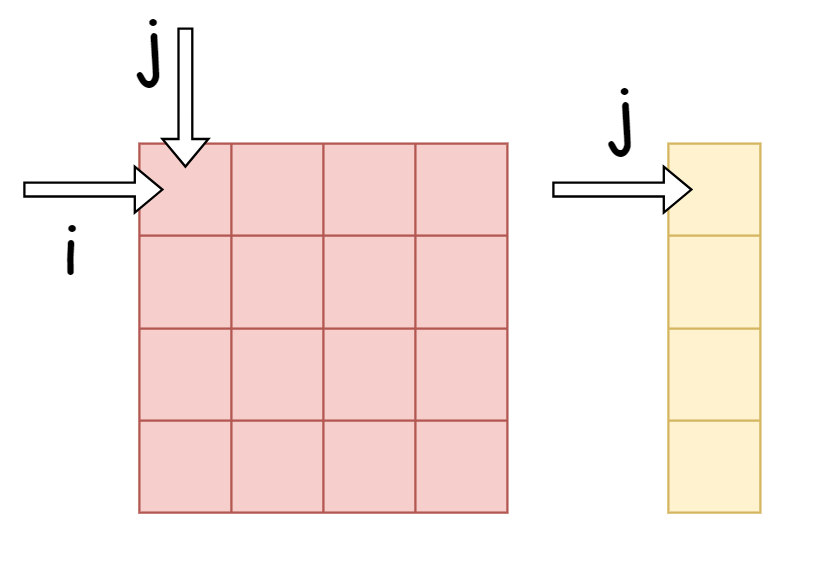
\includegraphics[width=0.4\linewidth]{PrimaItr.png}
    \caption{Primo passo}
    \label{fig:enter-label}    
\end{figure}
\begin{figure}[h]
    \centering
    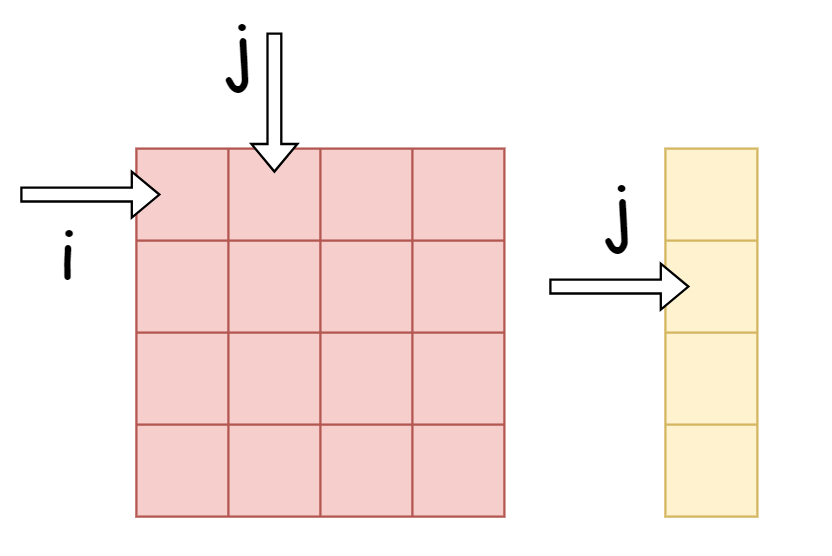
\includegraphics[width=0.4\linewidth]{SecondaItr.png}
    \caption{Secondo passo}
    \label{fig:enter-label}    
\end{figure}
\begin{figure}[h]
    \centering
    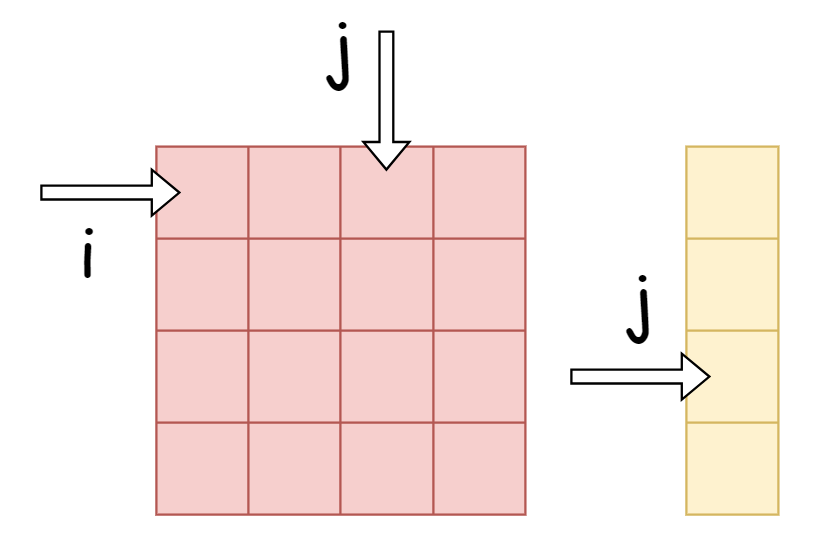
\includegraphics[width=0.4\linewidth]{Terza.png}
    \caption{Terzo passo}
    \label{fig:enter-label}    
\end{figure}
\begin{figure}[h]
    \centering
    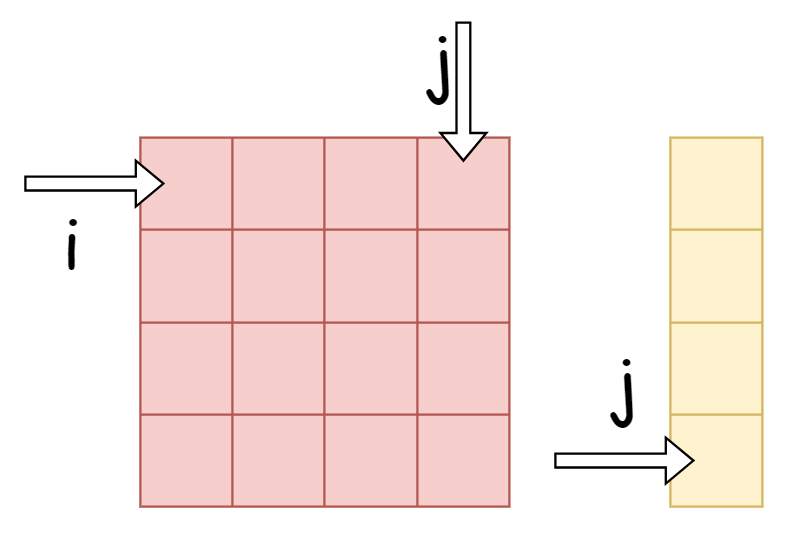
\includegraphics[width=0.4\linewidth]{QuartaItr.png}
    \caption{Quarto passo}
    \label{fig:enter-label}    
\end{figure}
\begin{figure}[h]
    \centering
    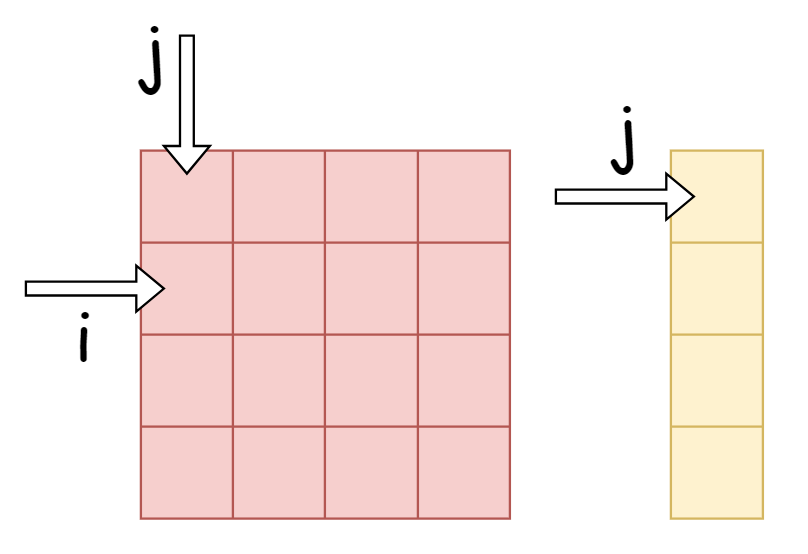
\includegraphics[width=0.4\linewidth]{QuintaItr.png}
    \caption{Quinto passo}
    \label{fig:enter-label}    
\end{figure}
e così via.

\subsection{Approccio alla risoluzione del problema dato}
Si può facilmente notare che i passi dell'algoritmo sono perfettamente indipendenti tra loro: ciò significa che è possibile una loro suddivisione tra esecutori.

La suddivisione proposta sfrutta la API (Application Programming Interface DA METTERE COME NOTA) OpenMP, la quale permette la parallelizzazione in calcolatori MIMD a memoria condivisa mediante la suddivisione di un processo in thread.

\section{strategia di parallelizzazione}


\clearpage
\section{Implementazione dell'algoritmo}

\subsection{Header file richiamati}
\begin{lstlisting}
#include <stdio.h>
#include <stdlib.h>
#include <omp.h>
\end{lstlisting}

\subsection{Implementazione}
\begin{lstlisting}
double *matrixVector(int m,int n,double *x,double **A);
double **readMatrixFromFile(char *path,int *m,int *n);
double *readVector(char *path,int *m);
void printVector(double *y,int m);
\end{lstlisting}

\subsection{Main}
\begin{lstlisting}
int main(){
    int m,n;
    double **A=readMatrixFromFile("/homes/DMA/PDC/2024/TRTFNC03B/mat_vet_omp/matrice.txt",&m,&n);

    int m2;
    double *x=ltor("/homes/DMA/PDC/2024/TRTFNC03B/mat_vet_omp/vettore.txt",&m2);

    if(m2!=n){
        printf("Vettore e matrice non hanno dimensioni adeguate per una moltiplicazione...");
        exit(-1);
    }
    else{
        double *y=matrixVector(m,n,x,A);
        printVector(y,m);
    }

}
\end{lstlisting}


\subsection{Prodotto matrice x vettore}

\begin{lstlisting}
double *matrixVector(int m,int n,double *x,double **A){
    
    double *y=calloc(m,sizeof(double));
    int i,j;
    #pragma omp parallel for default(none) shared(m,n,x,A,y) private(i,j)
        for(i=0;i<m;i++){
            for(j=0;j<n;j++){
                y[i]+=A[i][j]*x[j];
            }
        }
    return y;
}
\end{lstlisting}


\subsection{lettura Matrice}

\begin{lstlisting}
double **readMatrixFromFile(char *path,int *m,int *n){
    FILE *fp;
    fp=fopen(path,"r");
    int i,j;

    fscanf(fp,"%d %d",m,n);

    double **A=malloc((*m)*sizeof(double *));
    for(i=0;i<(*m);i++)
        A[i]=malloc((*n)*sizeof(double));

    
    for(i=0;i<(*m);i++){
        for(j=0;j<(*n);j++){
            fscanf(fp,"%lf",&(A[i][j]));
        }
    }

    fclose(fp);
    return A;

}
\end{lstlisting}

\subsection{Lettura vettore}

\begin{lstlisting}
double *readVector(char *path,int *m){
    FILE *fp;
    fp=fopen(path,"r");
    int i;
    fscanf(fp,"%d",m);

    double *x=malloc((*m)*sizeof(double));

    for(i=0;i<(*m);i++){
        fscanf(fp,"%lf",x+i);
    }
    fclose(fp);
    return x;
}
\end{lstlisting}

\subsection{Stampa vettore}

\begin{lstlisting}
void printVector(double *y,int m){
    int i;
    for(i=0;i<m;i++){
        printf("%f ",y[i]);
    }
    printf("\n");
}
\end{lstlisting}

\subsection{Misura istante iniziale}

\begin{lstlisting}

\end{lstlisting}

\subsection{Somma parallelizzata}

\begin{lstlisting}

\end{lstlisting}

\subsection{Blocco if strategia}

\begin{lstlisting}

\end{lstlisting}

\subsection{Presa tempo totale}

\begin{lstlisting}

\end{lstlisting}

\subsection{Stampa dei risultati}

\begin{lstlisting}
 ù
\end{lstlisting}


\section{Analisi dei tempi di esecuzione}
\subsection{Tempo di esecuzione}


\subsection{Speed-up, Overhead ed Efficienza}


\subsection{Speed-up scalato e isoefficienza}

\section{Modalità d'uso}



\end{document}
